\section{Diagrammes de s�quences}

\subsection{CU1}

\begin{center}
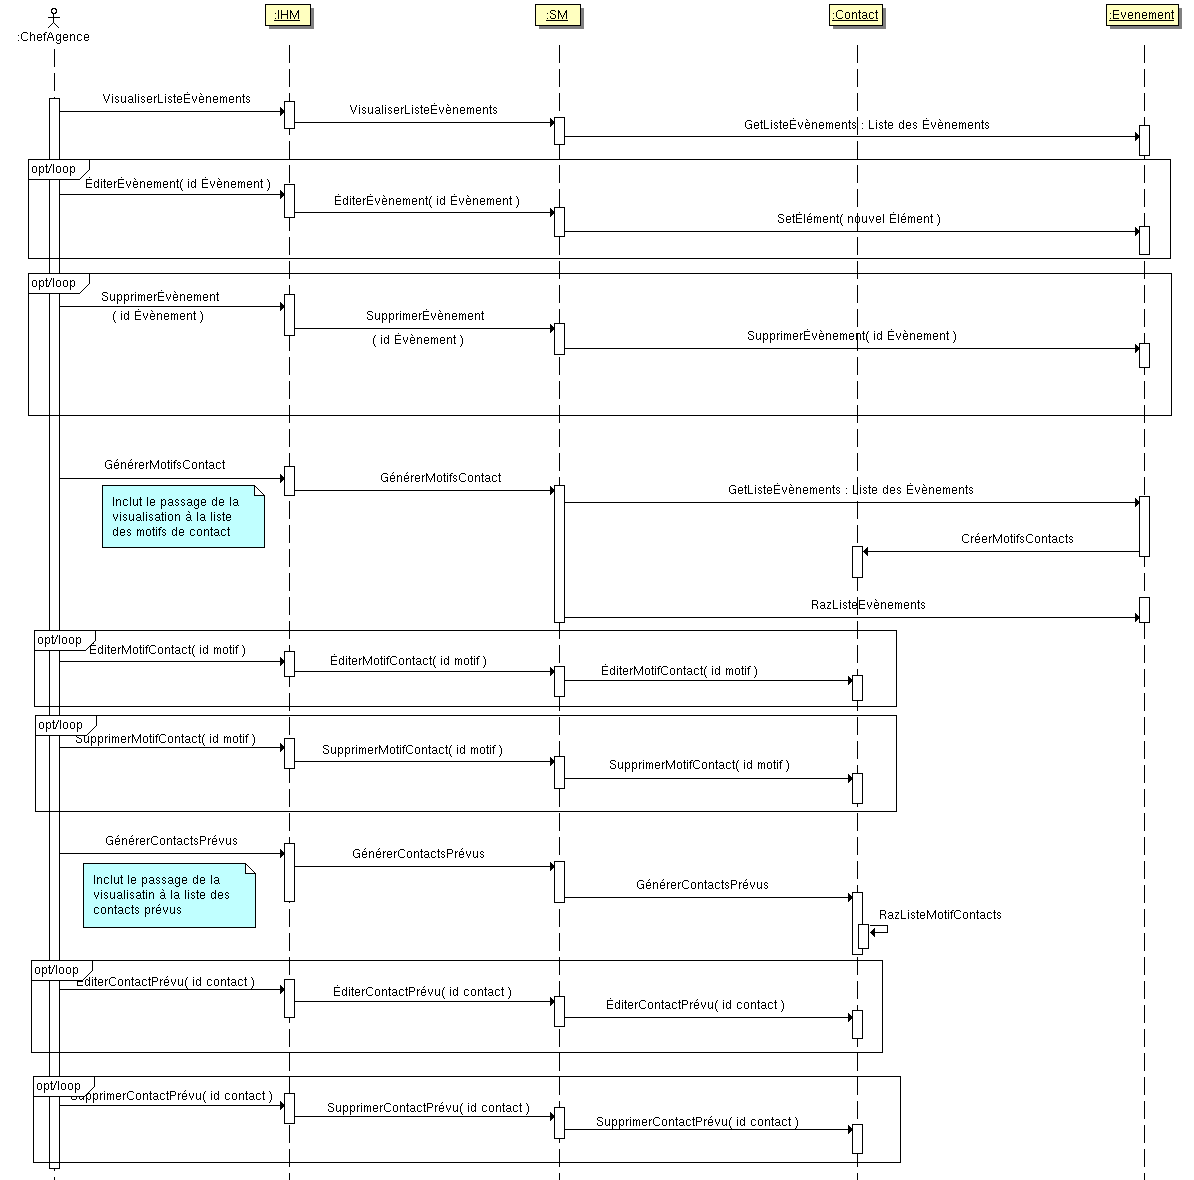
\includegraphics[width=15cm]{\PIXPATH/SD01}
\end{center}

\subsection{CU2}

\begin{center}
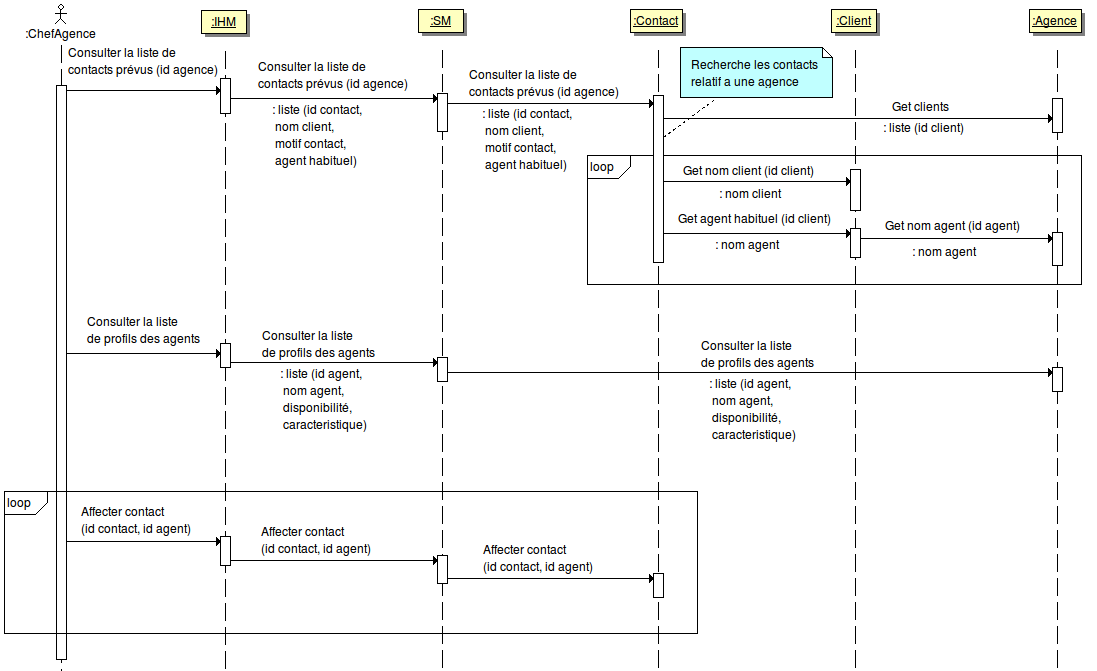
\includegraphics[width=15cm]{\PIXPATH/SD02}
\end{center}

\subsection{CU3}

\begin{center}
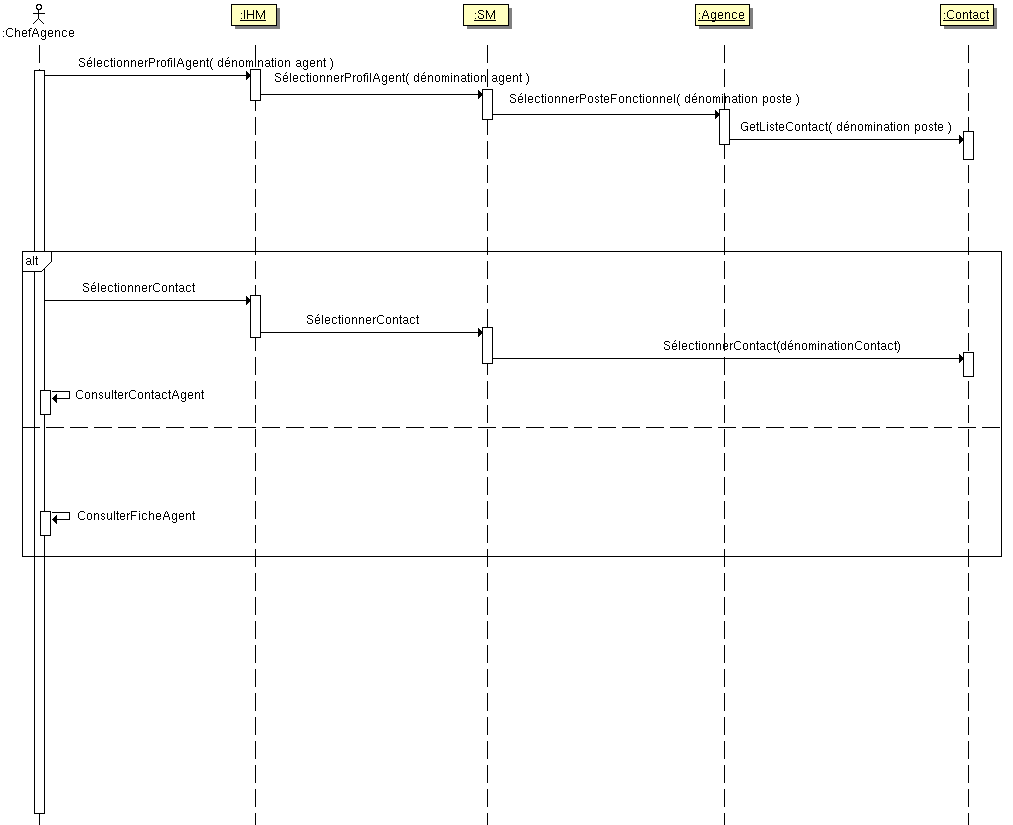
\includegraphics[width=15cm]{\PIXPATH/SD03}
\end{center}

\subsection{CU4}

\begin{center}
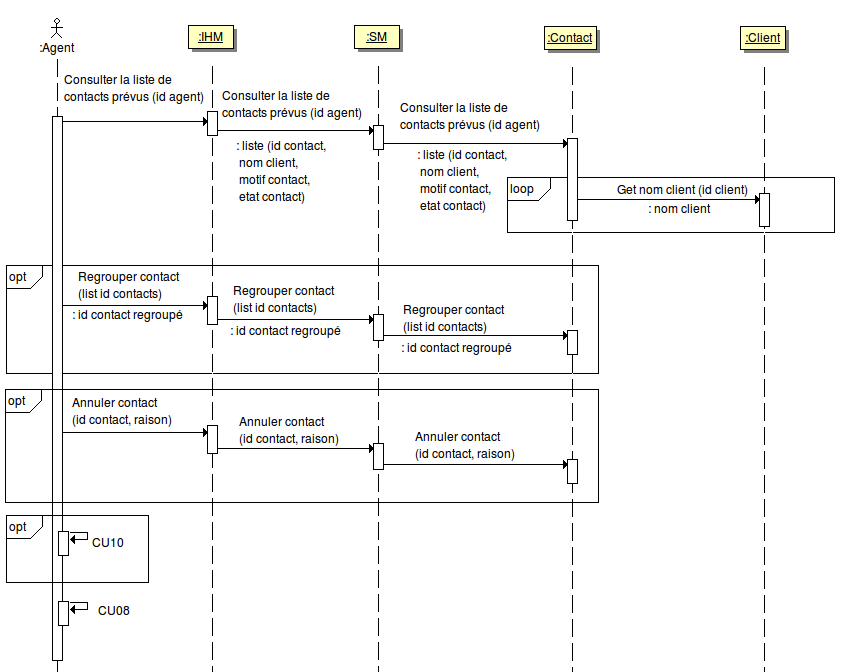
\includegraphics[width=15cm]{\PIXPATH/SD04}
\end{center}


\subsection{CU5}

\begin{center}
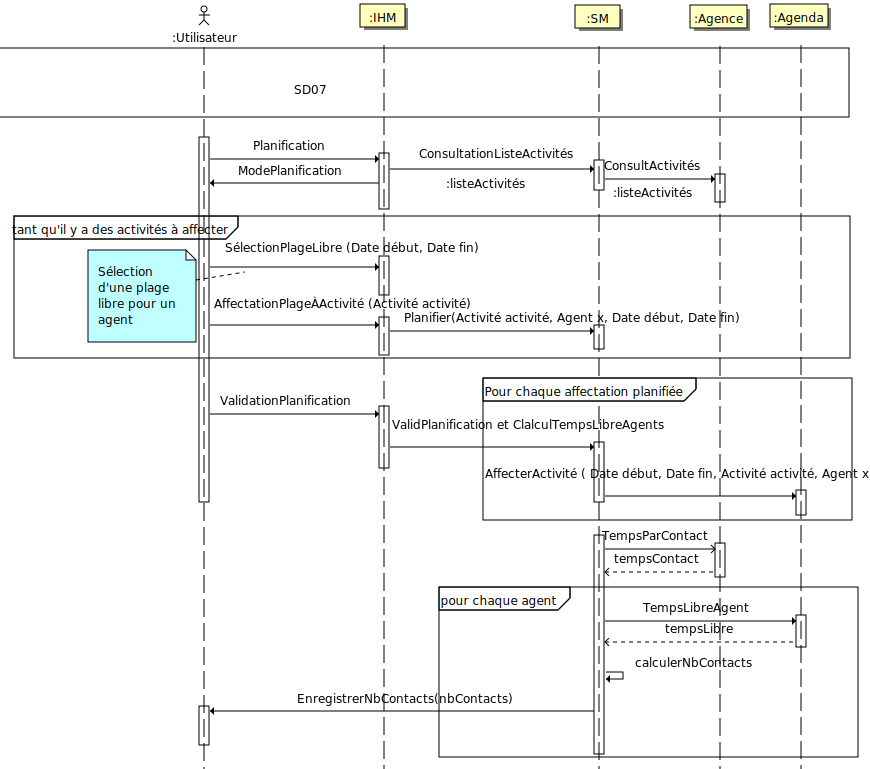
\includegraphics[width=15cm]{\PIXPATH/SD05}
\end{center}

\subsection{CU6}

\begin{center}
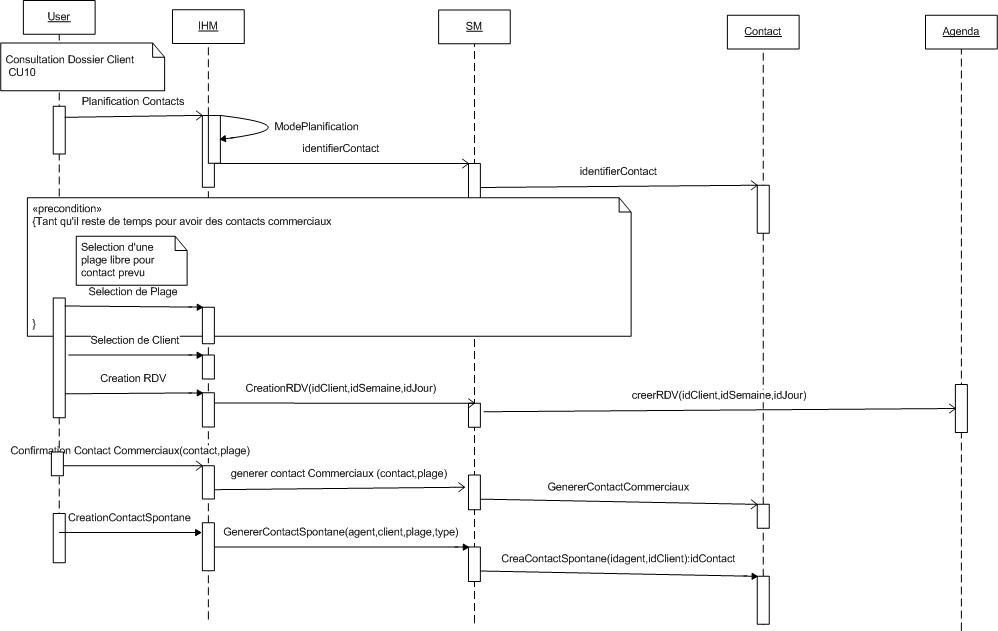
\includegraphics[width=15cm]{\PIXPATH/SD06}
\end{center}

\subsection{CU7}

\begin{center}
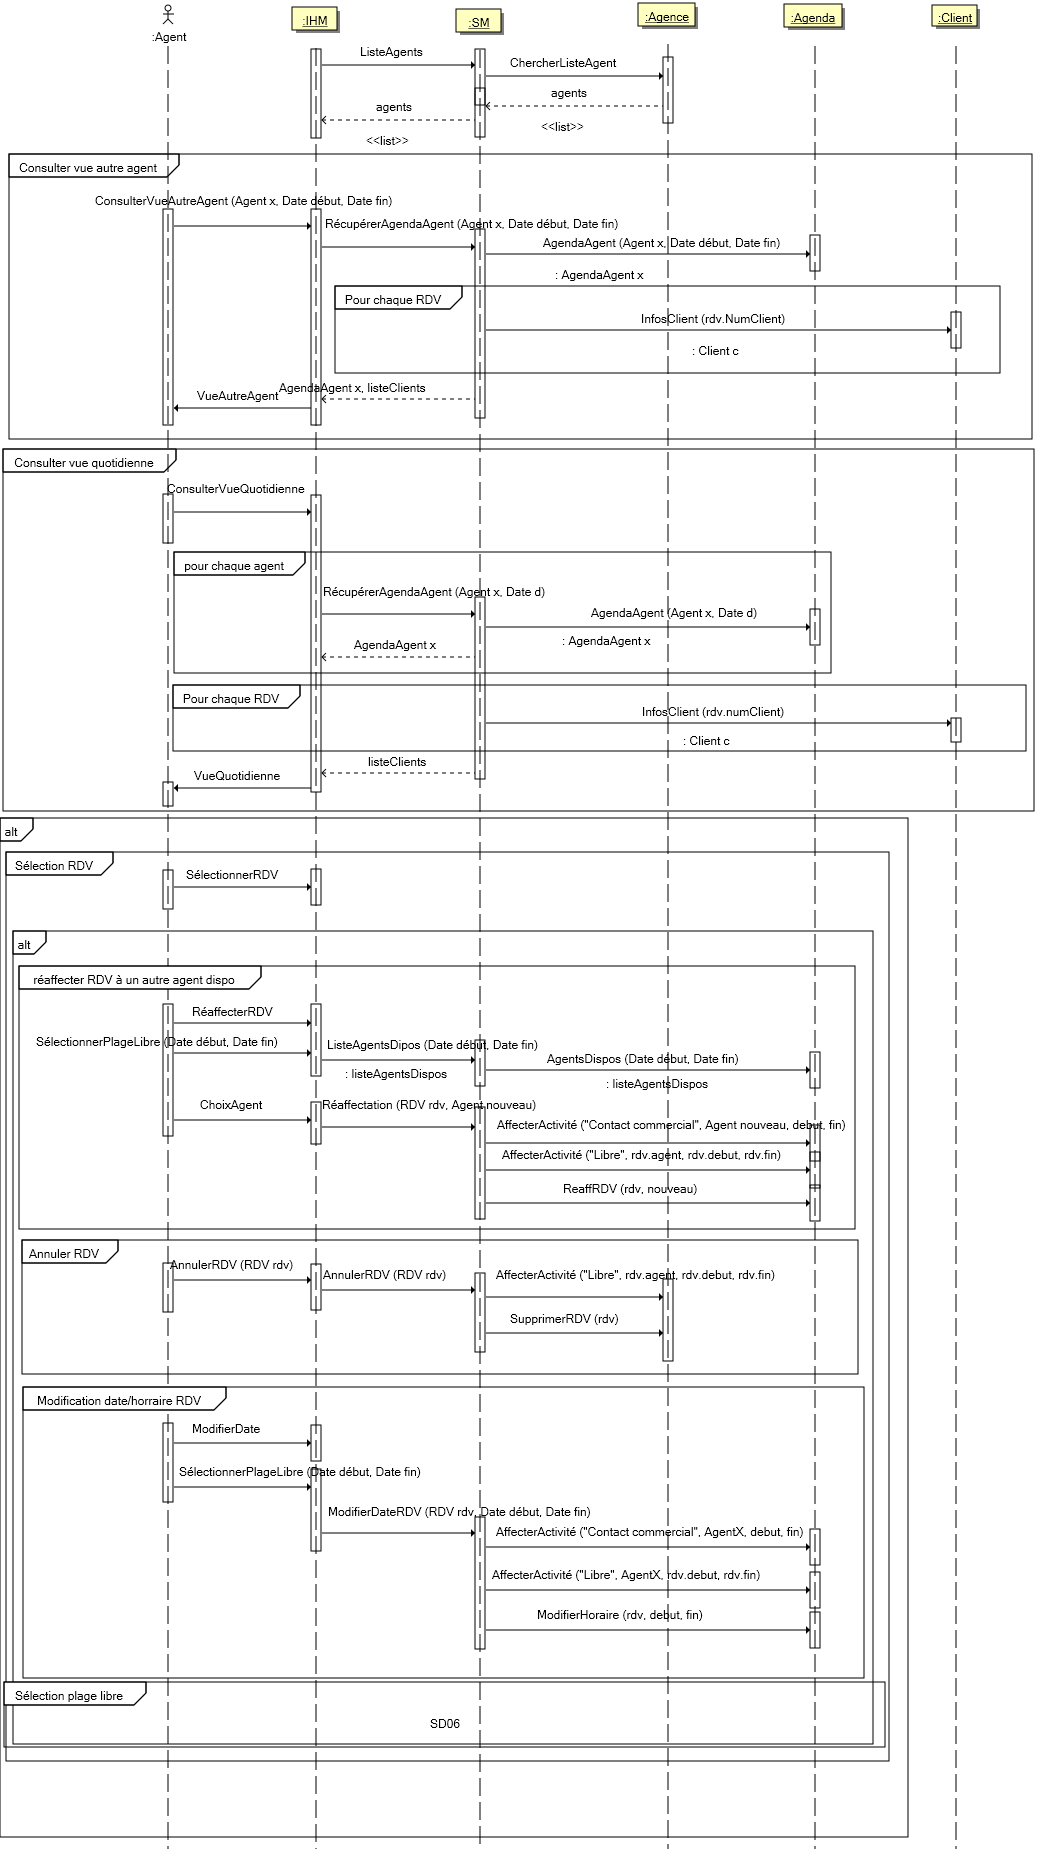
\includegraphics[width=15cm]{\PIXPATH/SD07}
\end{center}

\subsection{CU8}

\begin{center}
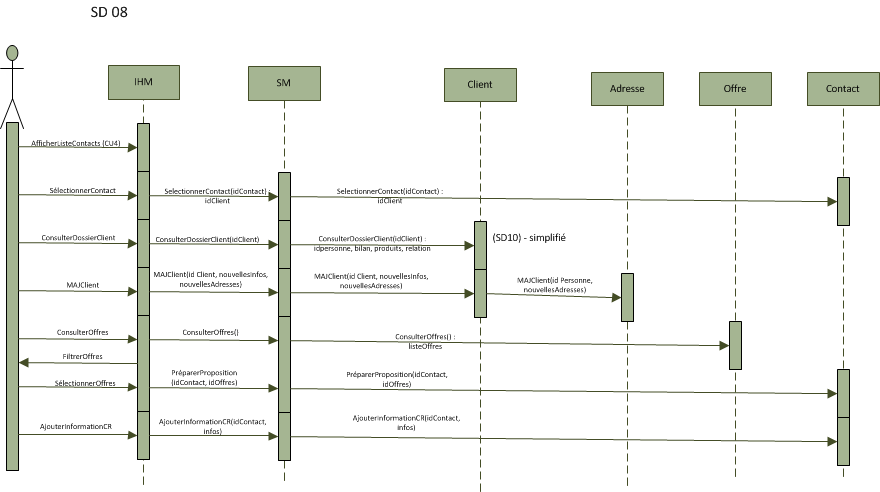
\includegraphics[width=15cm]{\PIXPATH/SD08}
\end{center}

\subsection{CU9}

\begin{center}
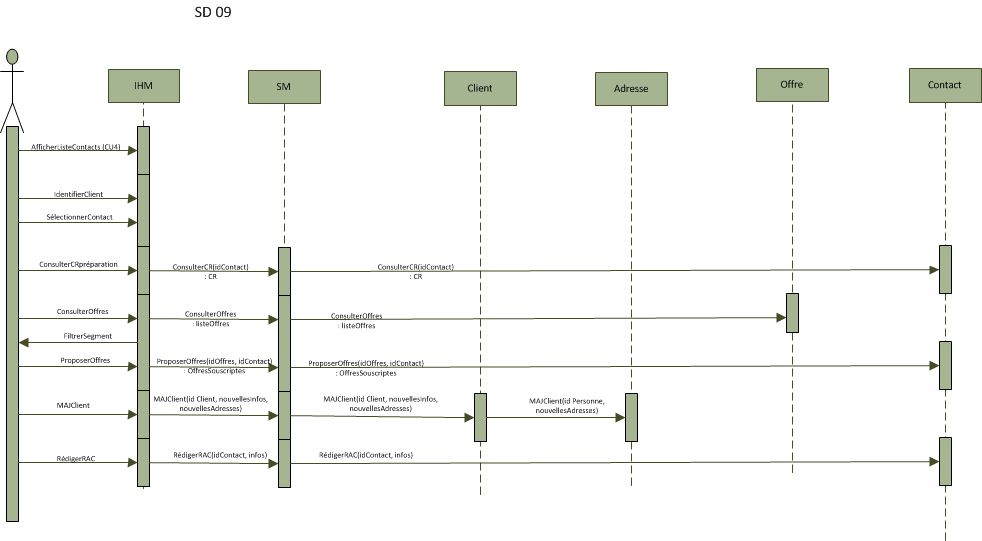
\includegraphics[width=15cm]{\PIXPATH/SD09}
\end{center}

\subsection{CU10}

\begin{center}
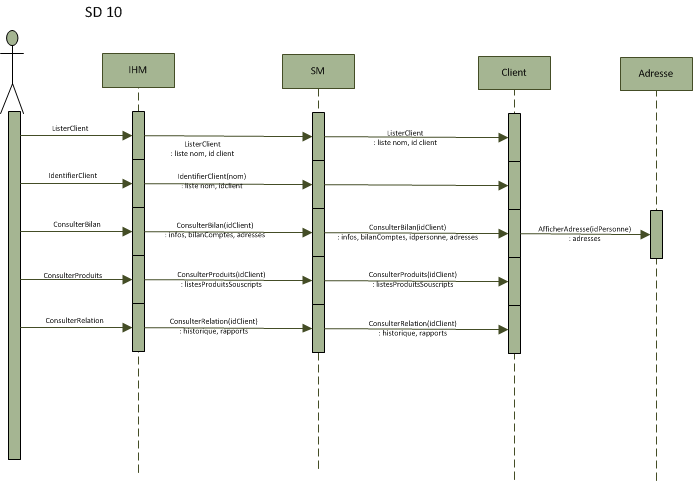
\includegraphics[width=15cm]{\PIXPATH/SD10}
\end{center}
